\chapter{Handlungsempfehlungen}\label{ch:empfehlungen}


\section{Anpassung der Unternehmensprozesse}\label{sec:anpassung-unternehmensprozesse}

Die in Kapitel~\ref{sec:gaps-auswirkungen} quantifizierten Gaps wurden zwar simulativ erzeugt, entsprechen aber Konfigurations- und Organisationsmustern, wie sie in Praxisberichten zu \gls{sap}-Anwender\-unternehmen wiederkehrend beschrieben werden\footcites(Vgl.)()[S.~3 ff.]{reinkemeyer2020processmining}[S.~21 ff.]{peters2019processmining}. Dieses Kapitel leitet ab, wie ein Unternehmen die gemessenen Ineffizienzen beheben kann, gegliedert nach organisatorischen Maßnahmen, Customizing und Erweiterungen.

Auf organisatorischer Ebene setzen drei Maßnahmen an den Wurzeln der Muster an. Erstens eine Stammdaten-Governance. Für Kundenstammdaten werden Pflichtattribute, Verantwortlichkeiten und ein Bereinigungsprojekt definiert. Das Projekt identifiziert und klassifiziert die Datenquellen, bereinigt die Bestände und überwacht die Qualität kontinuierlich. Vollständige Versanddaten und Incoterms entziehen den Liefersperren (G3) die Grundlage. Zweitens die Entlastung der Auftragserfassung, etwa durch elektronischen Datenaustausch mit den umsatzstärksten Kunden. Das reduziert Erfassungsfehler und damit die Änderungsschleife (G2). Drittens ein definierter Reklamationsprozess mit Rollen und Fristen, der die Gutschrifts- und Nachlieferungsfälle (G6) aus der informellen E-Mail-Bearbeitung in einen messbaren Ablauf überführt. Dass Stammdatenmängel der zentrale Engpasstreiber im \gls{o2c}-Prozess sind, bestätigt die Fallstudie von Adolfsson/Saleh, in der fehlerhafte Kundenstammdaten bei einem Kunden in allen Fällen manuelle Lieferterminänderungen und in rund einem Fünftel nachträgliche Preiskorrekturen erzwangen\footcite[Vgl.][S.~55 f.\ und 61]{adolfsson2026o2c}. Automatisierung, Datenintegration und fortgeschrittene Analytik gelten in der Literatur übergreifend als zentrale Hebel zur Verbesserung des \gls{o2c}-Prozesses in \gls{sap} \gls{sd}\footcite[Vgl.][S.~110 ff.]{nadukuru2024o2c}. Diese organisatorischen Maßnahmen sind Voraussetzung dafür, dass die anschließenden Systemeinstellungen überhaupt greifen. Eine automatisierte Kreditprüfung ist nur so gut wie die zugrunde liegenden Kreditstammdaten, und eine Pflichtfeldsteuerung für Versanddaten verhindert Liefersperren nur dann, wenn zugleich definiert ist, wer die fehlenden Attribute in welcher Frist pflegt. Organisatorische und technische Maßnahmen bilden also keine Alternative, sondern greifen ineinander. Praktisch beginnt eine Stammdaten-Governance mit der Benennung von Verantwortlichen je Datenobjekt, der Definition verbindlicher Pflichtfelder und Pflegestandards sowie einem einmaligen Bereinigungslauf, der Dubletten und veraltete Einträge entfernt. Erst danach greifen die Pflichtfeldprüfungen im System, ohne den laufenden Betrieb zu blockieren.

\section{Customizing im \gls{sap}-System}\label{sec:customizing}

Der Großteil der Gaps lässt sich ohne Programmierung im Customizing schließen, Tabelle~\ref{tab:massnahmenkatalog} ordnet jedem Gap die Maßnahme und den \gls{sap}-Bezug zu. Kern ist die Automatisierung der Kreditprüfung im \gls{sap} Credit Management. Bestandskunden mit gutem Zahlungsverhalten erhalten regelbasierte Scores und Limits, sodass Sperren nur noch bei tatsächlichen Risikofällen entstehen (G1). Die Unvollständigkeitsprüfung und Pflichtfeldsteuerung verhindert Aufträge mit fehlenden Versanddaten (G3), die Umstellung des Fakturavorrats auf tägliche Läufe beseitigt die künstliche Wartezeit vor der Rechnungsstellung (G4), und ein restriktives Berechtigungskonzept für manuelle Preisänderungen erzwingt die Pflege im Konditionsstamm (G5). Nachträgliche Auftragsänderungen (G2) werden durch eine entlastete, fehlerärmere Auftragserfassung gesenkt, insbesondere durch die \gls{edi}-Anbindung der umsatzstärksten Kunden (M6)\footcite[Vgl.][S.~110 ff.]{nadukuru2024o2c}.

\begin{table}[!htb]
\centering
\caption{Maßnahmenkatalog mit Gaps, Lösungsansätzen und \gls{sap}-Bezug}\label{tab:massnahmenkatalog}
\small
\begin{tabularx}{\textwidth}{@{}>{\RaggedRight\arraybackslash}p{3.0cm} >{\RaggedRight\arraybackslash}p{2.8cm} >{\RaggedRight\arraybackslash}p{4.4cm} >{\RaggedRight\arraybackslash}p{3.9cm}@{}}
\toprule
\textbf{Maßnahme} & \textbf{Typ} & \textbf{\gls{sap}-Bezug} & \textbf{Adressiertes Gap /\allowbreak{} erwarteter Effekt} \\
\midrule
M1 Automatisierte Kreditprüfung & Customizing & \gls{sap} Credit Management: Scoring-Regeln, Limitprofile, Ausnahmeliste & G1: Sperrquote von 34,1 \% deutlich reduziert; Median-Liegezeit 1,9 AT entfällt für Bestandskunden \\
M2 Stammdatenbereinigung u. Pflichtfelder & organisatorisch + Customizing & Unvollständigkeitsprüfung, Pflichtfeldsteuerung, Geschäftspartnerpflege & G3: Liefersperrenquote von 12,3 \% Richtung Restrisiko; 3,9 $\rightarrow$ 0,8 AT bis Lieferbeleg \\
M3 Tägliche Fakturierungsläufe & Customizing & Fakturavorrat (VF04/\allowbreak{}VF06) als täglicher Hintergrundjob & G4: Liegezeit WA $\rightarrow$ Faktura von 2,6 auf ca. 0,5 AT \\
M4 Konditionspflege u. Berechtigungen & Customizing + organisatorisch & Preisfindung/\allowbreak{}Konditionstechnik, Rollenkonzept & G5: Fakturasperren (7,9 \%) weitgehend vermieden \\
M5 Workflow Reklamation/\allowbreak{}Gutschrift & Customizing/\allowbreak{}Workflow & Freigabeworkflow für Gutschriftsanforderungen & G6: definierte Durchlaufzeit, Transparenz \\
M6 \gls{edi}-Anbindung Top-Kunden & Erweiterung & \gls{idoc}-Eingang für Bestellungen (ORDERS) & G2: Änderungsquote (22,7 \%) sinkt; weniger Erfassungsfehler \\
\bottomrule
\end{tabularx}
\end{table}

Am Beispiel der Kreditprüfung (M1) lässt sich der Hebel konkretisieren. Im Ist-Zustand wird jeder Auftrag, der ein statisches Kreditlimit überschreitet, gesperrt und manuell freigegeben, unabhängig vom tatsächlichen Risiko. Das \gls{sap} Credit Management ordnet Kunden stattdessen Risikoklassen mit eigenen Prüfregeln und Limits zu, sodass Bestandskunden mit tadellosem Zahlungsverhalten automatisch freigegeben werden, während echte Risikofälle weiterhin geprüft werden. Die Sperre wird damit vom Regelfall zur Ausnahme, ohne den Schutz vor Forderungsausfällen aufzugeben. Zu beachten ist, dass mehrere Maßnahmen ineinandergreifen. M1 setzt gepflegte Kreditstammdaten voraus und der Verzicht auf manuelle Preise (M4) einen vollständigen Konditionsstamm. Die Stammdaten-Governance aus Kapitel~\ref{sec:anpassung-unternehmensprozesse} ist damit nicht eine Maßnahme unter mehreren, sondern das Fundament, auf dem die technischen Anpassungen aufbauen.

Über die Kreditprüfung hinaus greifen die übrigen Customizing-Maßnahmen an klar umrissenen Konfigurationspunkten an. Die Unvollständigkeitsprüfung wird so eingestellt, dass ein Auftrag ohne gepflegte Versanddaten gar nicht erst zur Lieferung freigegeben wird, was die Liefersperren an der Wurzel verhindert. Der Fakturavorrat wird von einem wöchentlichen auf einen täglichen Hintergrundjob umgestellt, und die Berechtigung, Preise manuell im Auftrag zu überschreiben, wird auf wenige Rollen beschränkt, sodass Sonderkonditionen künftig im Konditionsstamm gepflegt werden. Keine dieser Einstellungen erfordert eine Programmierung, sie nutzen ausschließlich vorgesehene Parameter des Standards, was Wartbarkeit und Release-Fähigkeit erhält.

\section{Erweiterungen und kontinuierliches Monitoring}\label{sec:modifikationen-monitoring}

Eigenentwicklungen oder Modifikationen des \gls{sap}-Standards sind für keines der sechs Gaps erforderlich, im Einklang mit dem bewährten Grundsatz möglichst großer Standardnähe. Als Erweiterung im Sinne des Enhancement-Typs des Process Mining empfiehlt sich jedoch ein kontinuierliches Prozessmonitoring. Die Extraktionslogik aus Kapitel~\ref{sec:logkonstruktion} wird als wiederkehrender Ladeprozess eingerichtet, sodass Kennzahlen wie Sperrquoten, Liegezeiten und Happy-Path-Anteil laufend überwacht und Maßnahmenwirkungen gemessen werden können. Process Mining wandelt sich damit von einer einmaligen Diagnose zu einem dauerhaften Steuerungsinstrument\footcite[Vgl.][S.~3 ff.]{reinkemeyer2020processmining}. Die verwendete Werkzeugkette aus Python und \gls{pm4py} zeigt, dass dafür nicht zwingend eine kommerzielle Plattform erforderlich ist, wie sie \gls{sap} mit dem Beispielinhalt „Process Mining on \gls{sap} \gls{s/4hana}“ in \gls{papm} für dasselbe Szenario anbietet\footcite[Vgl.][Abschnitt~2.1, S.~9]{sap2022samplecontent}.

Der Aufbau eines solchen Monitorings ist selbst ein kleines Datenprojekt. Die Extraktion muss regelmäßig und möglichst inkrementell erfolgen, die Kennzahlen sind in einem Dashboard zu verdichten, und für kritische Größen wie eine wieder steigende Sperrquote sind Schwellenwerte für Warnungen festzulegen. Damit wird aus der einmaligen Fit/Gap-Analyse ein geschlossener Regelkreis, in dem Abweichungen früh erkannt und gegengesteuert werden, bevor sie sich in Durchlaufzeit und Forderungslaufzeit niederschlagen. Konkret bieten sich als Kennzahlen die bereits in der Analyse verwendeten Größen an, also die Sperrquoten je Sperrentyp, die Median-Liegezeiten je Prozessübergang, der Anteil konformer Fälle und die Durchlaufzeit bis zur Faktura. Werden sie zusätzlich je Verkaufsorganisation oder Kundengruppe aufgeschlüsselt, lassen sich Problembereiche gezielt eingrenzen, statt nur einen Gesamtdurchschnitt zu betrachten.

\section{Implementierungsstrategie}\label{sec:schrittweise-umsetzung}

Die Umsetzung der Maßnahmen wird in die etablierten Phasen einer \gls{erp}-Anpassung gegliedert. Diese umfassen Projektplanung, Systemkonfiguration, Datenbereinigung, Testphase, Schulung und Go-Live. Insgesamt ist sie auf sechs Monate ausgelegt (Abbildung~\ref{fig:implementierungsplan}). Nach dem Detailkonzept (P1) laufen die Stammdatenbereinigung (P2) und das Customizing des Kreditmanagements (P3) parallel. Die Umstellung der Fakturierungsläufe (P4) ist bewusst früh terminiert, weil sie mit geringem Aufwand die größte Liquiditätswirkung entfaltet („Quick Win“, Abbildung~\ref{fig:liegezeiten}). Es folgen der Gutschriften-Workflow (P5), Integrationstests und Schulungen (P6) sowie Go-Live mit Hypercare-Phase (P7). Die Planung nutzt die klassischen Instrumente Projektstrukturplan, Meilensteine und Gantt-Diagramm.

\begin{figure}[!htb]
\centering
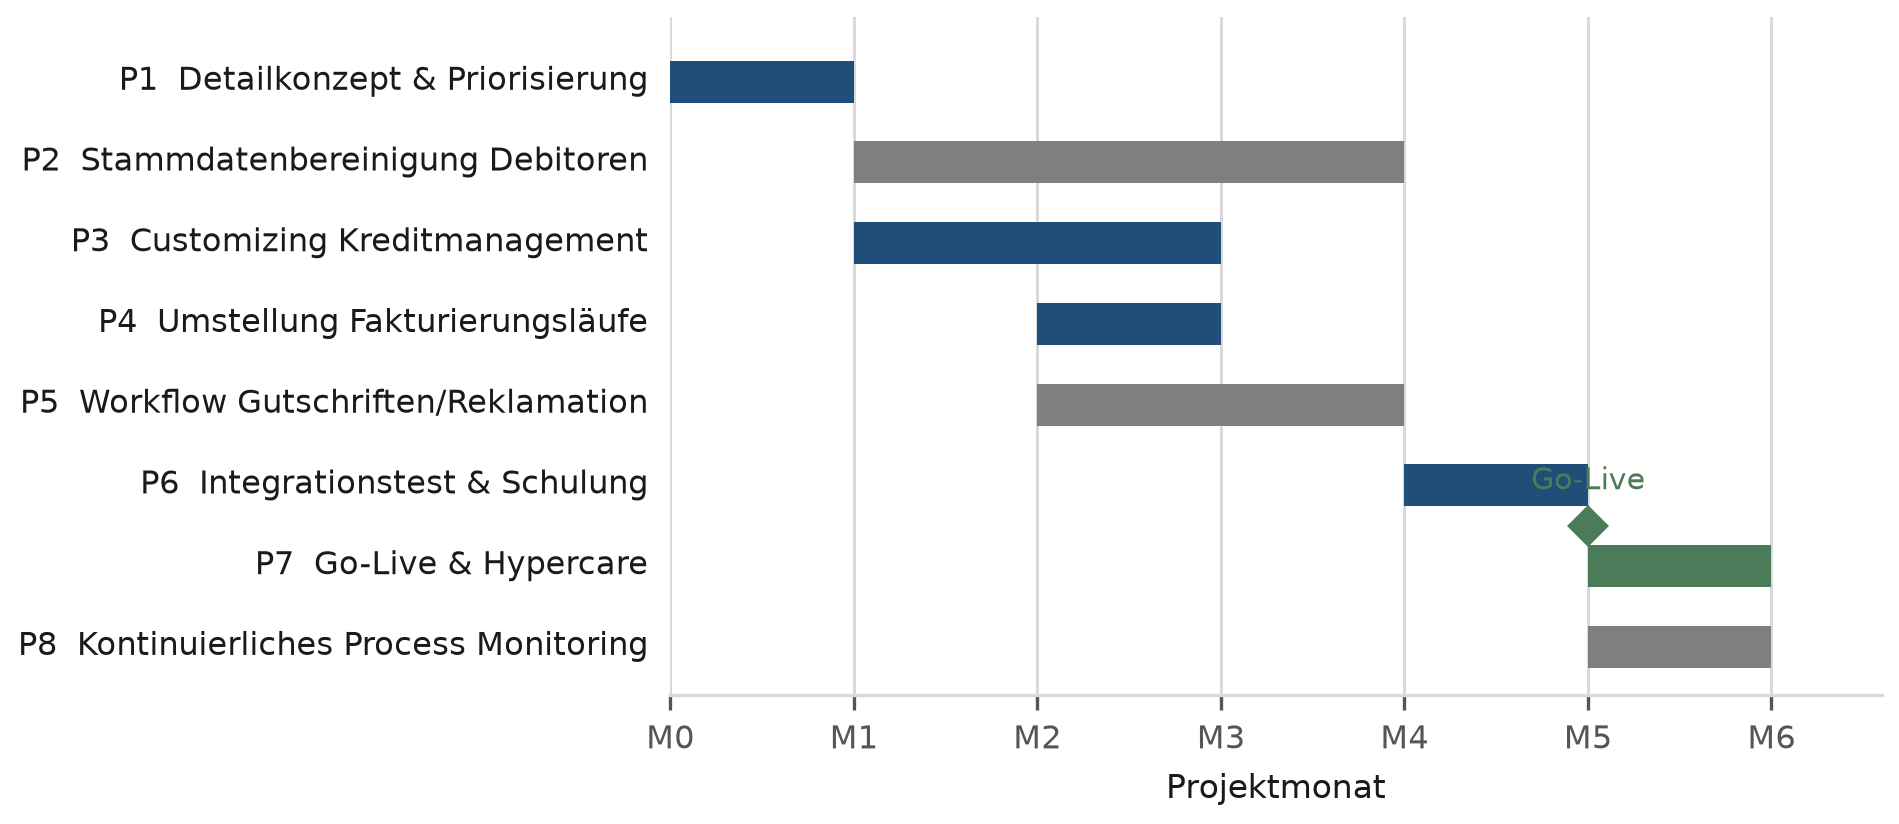
\includegraphics[width=\textwidth,height=0.36\textheight,keepaspectratio]{figures/image7.png}
\caption{Implementierungsplan über sechs Monate}\label{fig:implementierungsplan}
\end{figure}

Ein iteratives, phasenweises Vorgehen ist auch aus Risikosicht geboten. Statt alle sechs Maßnahmen gleichzeitig produktiv zu setzen, werden sie nacheinander eingeführt und ihre Wirkung jeweils über das Prozessmonitoring gemessen, bevor die nächste folgt. So lässt sich etwa bei der automatisierten Kreditprüfung (M1) in einem Parallellauf beobachten, ob die neuen Regeln zu viele Aufträge blockieren oder umgekehrt Risikofälle durchlassen, und die Schwellenwerte können nachjustiert werden, bevor die manuelle Prüfung vollständig abgelöst wird. Dieses Vorgehen entspricht einem Phased Rollout und reduziert das Risiko, dass eine fehlerhafte Einstellung den gesamten \gls{o2c}-Prozess stört. Inhaltlich gliedert sich das Vorhaben damit in eine Vorbereitungsphase (Detailkonzept und Priorisierung anhand der gemessenen Kennzahlen), eine Umsetzungsphase (parallele Stammdatenbereinigung und Customizing mit dem Fakturalauf als frühem Quick Win) und eine Stabilisierungsphase (Integrationstest, Schulung, Go-Live und Hypercare). Der Übergang von einer Phase zur nächsten ist jeweils an ein messbares Ergebnis geknüpft, etwa eine gesunkene Sperrquote im Parallellauf. Die Gesamtdauer von sechs Monaten ergibt sich dabei weniger aus dem technischen Aufwand der einzelnen Einstellungen, der überschaubar ist, als aus der Stammdatenbereinigung, den Testzyklen und der notwendigen Eingewöhnung der Anwender.

Für die Testphase sind Integrations-, User-Acceptance- und Regressionstests mit realistischen Testdaten vorgesehen. Personell erfordert das Vorhaben eine interne Projektleitung (ca. 0,3 \gls{vzae}), je einen Key-User aus Vertrieb, Versand und Debitorenbuchhaltung (je ca. 0,2 \gls{vzae}), externe \gls{sd}-/\gls{fscm}-Beratung (ca. 25 Personentage) sowie die \gls{it} für Berechtigungen und Hintergrundjobs. Die externen Kosten lassen sich auf Basis marktüblicher Beratungstagessätze grob auf 60.000 bis 80.000 \euro{} schätzen. Dem stehen im modellierten Szenario rund 1.950 eingesparte Klärungsstunden pro Jahr (ca. 1,2 \gls{vzae}) sowie eine um mehrere Tage verkürzte Zeitspanne bis zur Rechnungsstellung gegenüber, die die Forderungslaufzeit unmittelbar senkt. Nach der \gls{roi}-Logik amortisiert sich das Vorhaben unter diesen Annahmen bereits im ersten Jahr. Nach dem Go-Live werden Erfolgskriterien als Post-Go-Live-Metriken definiert und in der Hypercare-Phase proaktiv überwacht, unmittelbar über das Prozessmonitoring aus Kapitel~\ref{sec:modifikationen-monitoring} mit den Kennzahlen aus Anhang III.

Die Testphase verdient dabei besondere Aufmerksamkeit, weil die Maßnahmen tief in den erlöswirksamen Prozess eingreifen. Neben den funktionalen Integrationstests sind Regressionstests der angrenzenden Prozesse in Beschaffung, Bestandsführung und Debitorenbuchhaltung vorzusehen, und die neuen Kreditregeln sind an einem repräsentativen Ausschnitt historischer Aufträge zu erproben, um Fehlsperren zu vermeiden. Erst nach erfolgreichem User-Acceptance-Test durch die Key-User erfolgt der Go-Live.

Wirtschaftlich ist das Vorhaben auch unter konservativen Annahmen tragfähig. Den einmaligen externen Kosten stehen wiederkehrende Effekte gegenüber, nämlich eingesparte Klärungsstunden, eine kürzere Forderungslaufzeit und eine höhere Liefertermintreue. Weil die Liquiditätswirkung der täglichen Fakturierung sofort und ohne laufende Kosten eintritt, während die Beratungskosten nur einmalig anfallen, verschiebt sich das Kosten-Nutzen-Verhältnis bereits im ersten Jahr deutlich ins Positive. Entscheidend für die Belastbarkeit dieser Rechnung ist, dass die zugrunde liegenden Ist-Werte aus der Analyse gemessen und nicht geschätzt sind, sodass die erwarteten Einsparungen an konkreten, nachprüfbaren Kennzahlen festgemacht werden können.

\section{Risiken und Veränderungsmanagement}\label{sec:risikobewertung}

Die Risiken des Vorhabens liegen weniger in der Technik als in Datenqualität, Organisation und Akzeptanz. Tabelle~\ref{tab:risikomatrix} bewertet die wichtigsten Risiken und hinterlegt Gegenmaßnahmen. Hervorzuheben ist das Datenschutzrisiko, das beim Übergang von synthetischen auf reale Event-Logs entsteht. Reale Logs enthalten Benutzerkennungen und erlauben Leistungs- und Verhaltensauswertungen, Betriebsrat und Datenschutzbeauftragte sind daher früh einzubinden, und die Analysen sind auf pseudonymisierte, nicht personenbezogene Auswertungen zu beschränken.

\begin{table}[!htb]
\centering
\caption{Risikomatrix der Implementierung}\label{tab:risikomatrix}
\small
\begin{tabularx}{\textwidth}{@{}Y l l Y@{}}
\toprule
\textbf{Risiko} & \textbf{Eintritt} & \textbf{Auswirkung} & \textbf{Gegenmaßnahme} \\
\midrule
Datenqualität schlechter als angenommen (Stammdaten) & hoch & mittel & frühe Testextraktion, Bereinigung priorisieren, Puffer in P2 \\
Zu scharfe Kreditregeln blockieren Aufträge /\allowbreak{} zu laxe erhöhen Forderungsausfälle & mittel & hoch & Pilotbetrieb mit Parallellauf, Schwellenwerte iterativ justieren, Ausnahmeliste \\
Akzeptanz: Mitarbeitende fühlen sich durch Prozessdaten überwacht (reale Logs) & mittel & hoch & Pseudonymisierung, Betriebsvereinbarung, transparente Kommunikation der Ziele \\
Scope-Ausweitung (weitere Prozesse „auch noch schnell“) & mittel & mittel & Change-Request-Verfahren, Priorisierung nach Nutzwert \\
Wissensabfluss nach Beratungsende & niedrig & mittel & Dokumentation, Key-User-Schulung, Betreuungsvereinbarung \\
\bottomrule
\end{tabularx}
\end{table}

Neben diesen sachlichen Risiken ist das Veränderungsmanagement entscheidend, weil die Maßnahmen etablierte Arbeitsweisen ablösen. Die Umstellung von der manuellen auf die automatisierte Kreditfreigabe etwa entzieht der Debitorenbuchhaltung eine gewohnte Kontrollaufgabe und muss durch frühzeitige Einbindung, transparente Kommunikation der Ziele und Schulung begleitet werden. Gerade weil Process Mining das tatsächliche Verhalten sichtbar macht, ist der offene Umgang mit den Ergebnissen, verbunden mit der klaren Zusage, die Auswertung nicht zur individuellen Leistungskontrolle zu nutzen, eine Voraussetzung für die Akzeptanz im Team.

\section{Erfahrungen und Empfehlungen für vergleichbare Projekte}\label{sec:erkenntnisse-empfehlungen}

Die Datenaufbereitung erwies sich als der eigentliche Engpass, selbst bei synthetischen Daten. In einer ersten Fassung des Simulationsmodells erzeugten nicht streng monotone Zeitstempel Schein-Kanten im entdeckten Modell. Solche Granularitäts- und Sortierprobleme treten auch bei realen \gls{sap}-Extraktionen auf, wenn tagesgenaue Felder wie \gls{augdt} mit sekundengenauen Zeitstempeln gemischt werden, und müssen vor der Discovery behoben werden, sonst analysiert man Artefakte statt Prozesse. Sie entsprechen den in der Literatur katalogisierten Imperfektionsmustern von Event-Logs, für die dort ein systematisches Bereinigungsvorgehen empfohlen wird\footcite[Vgl.][S.~132 ff.]{suriadi2017imperfection}. Konkret zeigte sich die Bedeutung der Datenaufbereitung daran, dass erst die Erzwingung streng monoton steigender Zeitstempel je Fall die scheinbaren Rücksprünge im Modell beseitigte. Dieses Detail wäre bei einer flüchtigen Betrachtung der Werkzeugausgabe leicht als echter Prozessschritt fehlgedeutet worden. Die Lehre daraus ist, dass die Plausibilität des Event-Logs vor jeder inhaltlichen Interpretation zu prüfen ist. Ebenso zeigte sich, dass die Methodenwahl kein akademisches Detail ist. Zwischen Alpha-Algorithmus und Inductive Miner lagen auf demselben Log deutliche Unterschiede (Fitness 0,646 gegenüber 0,996), und beim Soll-Abgleich machte erst der Wechsel vom Token-Replay zu Alignments die tatsächliche Konformität sichtbar (Kapitel~\ref{sec:gaps-auswirkungen}). Wer Werkzeugausgaben interpretiert, muss wissen, welcher Algorithmus mit welchen Parametern dahinterliegt. Eine zweite Grenze betrifft die Reichweite der Daten selbst. Ein Event-Log zeigt, \emph{was} geschehen ist, nicht \emph{warum}. In der Fallstudie von Adolfsson/Saleh blieb eine durchgängige manuelle Auftragsabstimmung mit dem Vertrieb unsichtbar, weil sie keine digitale Spur im \gls{erp}-System hinterließ\footcite[Vgl.][S.~50 und 62]{adolfsson2026o2c}. Für den synthetischen Log ist diese Grenze konstruktionsbedingt gegenstandslos, für die Übertragung auf reale Systeme jedoch zentral.

Daraus folgen vier Empfehlungen. Erstens sollten Kennzahlen wie Sperrquoten, Liegezeiten je Übergang, Happy-Path-Anteil und Zeit bis zur Faktura bereits vor der Analyse definiert werden. Ohne Ziel-\gls{kpi}s erzeugt Process Mining beeindruckende, aber folgenlose Visualisierungen. Zweitens verdient die Log-Qualitätsprüfung (Monotonie, Granularität, Vollständigkeit) einen festen Platz vor jeder Discovery. Drittens gehört beim Übergang auf reale Logs der Datenschutz an den Anfang, mit Pseudonymisierung der Benutzerkennungen und früher Einbindung von Betriebsrat und Datenschutzbeauftragten (Kapitel~\ref{sec:risikobewertung}). Viertens gilt der Grundsatz möglichst großer Standardnähe auch für die Behebung der Gaps. Alle sechs Maßnahmen kommen ohne Modifikation aus, was Wartbarkeit und Release-Fähigkeit erhält. Diese Empfehlungen decken sich mit der Praxisliteratur, die rät, Analysen breit-aggregiert zu beginnen, das Werkzeug mit Interviews und Workshops zu kombinieren und den Untersuchungsumfang zunächst eng zu fassen\footcite[Vgl.][S.~71 f.]{adolfsson2026o2c}. Eine fünfte Erkenntnis betrifft das Zusammenspiel von Methode und Fachwissen. Process Mining liefert präzise Diagnosen, aber keine Therapien. Die Entscheidung etwa, dass die Batch-Fakturierung trotz ihrer scheinbaren Harmlosigkeit die lohnendste erste Maßnahme ist, erfordert betriebswirtschaftliches Urteilsvermögen und Kenntnis des \gls{sap}-Customizings. Das datengetriebene Vorgehen ersetzt Prozessworkshops also nicht, es macht sie gezielter und beweisbarer\footcite[Vgl.][S.~71 f.]{adolfsson2026o2c}. Nicht zuletzt lohnt der Blick über den eigenen Prozess hinaus. Die Praxisliteratur und die herangezogene Fallstudie zeigen übereinstimmend, dass die größten Effekte weniger in ausgefeilteren Algorithmen als in sauberen Stammdaten und klar geschnittenen Prozessen liegen\footcites(Vgl.)()[S.~110 ff.]{nadukuru2024o2c}[S.~71 f.]{adolfsson2026o2c}. Process Mining ist damit vor allem ein Instrument, um diese unspektakulären, aber wirksamen Hebel überhaupt sichtbar und ihre Behebung messbar zu machen.

Langfristig liegt der Wert weniger in der einmaligen Diagnose als in der Verstetigung. Da Simulation und Analyse vollständig skriptbasiert und reproduzierbar sind, lässt sich dieselbe Auswertung nach jeder Prozessänderung erneut ausführen, als kontinuierliches Monitoring mit den Kennzahlen aus Anhang III (Kapitel~\ref{sec:modifikationen-monitoring}). Für die Organisation verschiebt das die Diskussionsgrundlage dauerhaft von Einzelmeinungen zu gemessener Evidenz. Prozessverbesserung wird überprüfbar und Prozessverantwortung messbar. Erfahrungsgemäß entsteht daraus ein kultureller Wandel. Wo Kennzahlen sichtbar sind, kehren alte Muster wie schleichend zunehmende manuelle Preisänderungen seltener unbemerkt zurück, weil jede Abweichung im Monitoring auffällt. Perspektivisch ist die Übertragung auf weitere Belegflüsse wie den Purchase-to-Pay-Prozess angelegt, für den der \gls{bpi}-Challenge-2019-Log als öffentliches Übungsfeld bereitsteht\footcite[Vgl.][]{vandongen2019bpi}.
